\documentclass[tikz,border=10pt]{standalone}
\usepackage{amsmath}
\usepackage{tikz}
\usetikzlibrary{arrows.meta, positioning, calc, shapes.geometric}
\usepackage{xcolor}


\begin{document}
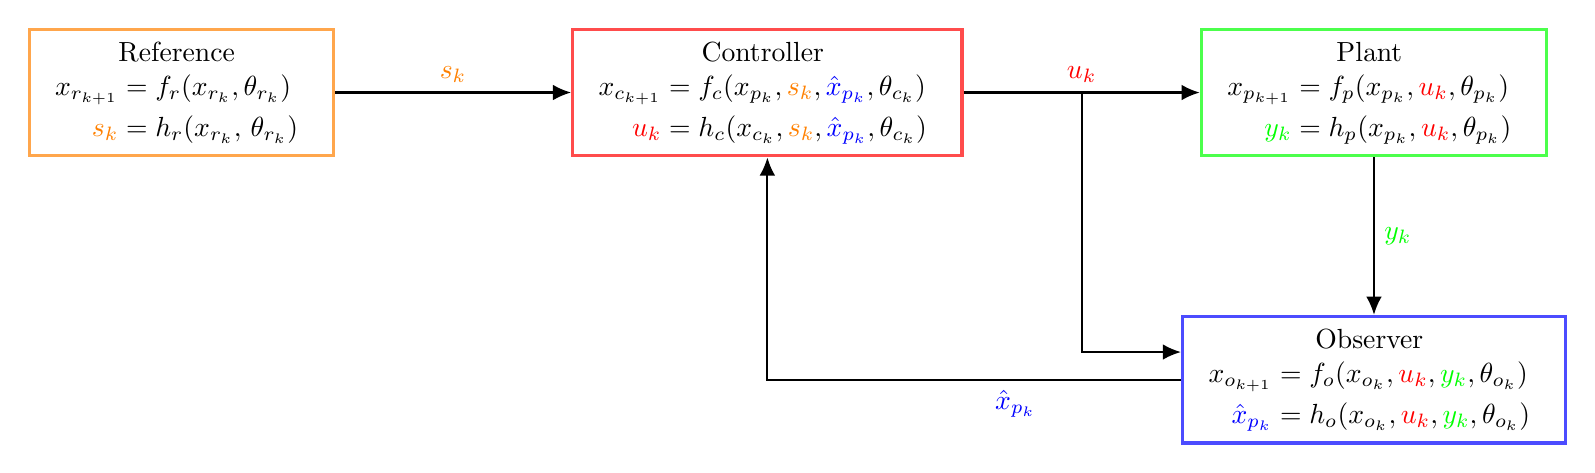
\begin{tikzpicture}[
  block/.style = {draw, thick, minimum height=3em, minimum width=6em, align=center},
  orangeblock/.style = {draw=orange!70, very thick, minimum height=3em, minimum width=6em, align=center},
  redblock/.style = {draw=red!70, very thick, minimum height=3em, minimum width=6em, align=center},
  greenblock/.style = {draw=green!70, very thick, minimum height=3em, minimum width=6em, align=center},
  blueblock/.style = {draw=blue!70, very thick, minimum height=3em, minimum width=6em, align=center},      
  arrow/.style = {thick, -{Latex[width=2mm]}},
  node distance=2.5cm and 2.5cm
]

  % ======================================================
  % Scenario 1 Setpoint (blue block)
  % ======================================================
  \node[orangeblock] (setpoint) {
    \begin{tabular}{c}
      Reference \\
      $\begin{aligned}
        x_{r_{k+1}} &= f_r(x_{r_k}, \theta_{r_k}) \\
        \textcolor{orange}{s_k} &= h_{r}(x_{r_k},\,\theta_{r_k})
      \end{aligned}$
    \end{tabular}
  };

  % PID Controller (to the right)
  \node[redblock, right=3.0cm of setpoint] (controller) {
    \begin{tabular}{c}
            Controller\\
      $\begin{aligned}
      x_{c_{k+1}} &= f_c(x_{p_{k}}, \textcolor{orange}{s_k}, \textcolor{blue}{\hat{x}_{p_k}},\theta_{c_k}) \\
      \textcolor{red}{u_k} &= h_c(x_{c_k}, \textcolor{orange}{s_k}, \textcolor{blue}{\hat{x}_{p_k}},\theta_{c_k})
       \end{aligned}$      
    \end{tabular}
  };

  % Plant
  \node[greenblock, right=3.0cm of controller] (system) {
    \begin{tabular}{c}
      Plant\\      
      $\begin{aligned}
      x_{p_{k+1}} &= f_p(x_{p_{k}}, \textcolor{red}{u_k}, \theta_{p_k}) \\
      \textcolor{green}{y_k} &= h_p(x_{p_{k}}, \textcolor{red}{u_k}, \theta_{p_k})
       \end{aligned}$                  
    \end{tabular}
  };

  % Observer (KF)
  \node[blueblock, below=2cm of system] (observer) {
    \begin{tabular}{c}
      Observer\\      
    $\begin{aligned}
      x_{o_{k+1}} &= f_o(x_{o_k}, \textcolor{red}{u_k}, \textcolor{green}{y_k}, \theta_{o_k}) \\
      \textcolor{blue}{\hat{x}_{p_k}} &= h_o(x_{o_k}, \textcolor{red}{u_k}, \textcolor{green}{y_k}, \theta_{o_k})
       \end{aligned}$            
    \end{tabular}
  };

  % r -> PID
  \draw[arrow] (setpoint.east) -- node[above] {$\textcolor{orange}{s_k}$} (controller.west);

  % controller -> plant
  \draw[arrow] (controller.east) -- node[above] {$\textcolor{red}{u_k}$} (system.west);

  % u branch to observer (split)
  \coordinate (usplit) at ($(controller.east)!0.5!(system.west)$);
  \coordinate[above=1em of observer.west] (observer_uin);
  \draw[arrow] (usplit) |- (observer_uin) node[pos=0.25, right] {};

  % y_p -> observer
  \draw[arrow] (system.south) -- node[right] {$\textcolor{green}{y_k}$} (observer.north);

  % observer -> controller (\hat{x}_k feedback)
  \coordinate (controller_yoin) at ($(controller.south)!0.5!(controller.south -| observer.north)$);
  \draw[arrow] (observer.west) -| node[pos=0.2, below] {$\textcolor{blue}{\hat{x}_{p_k}}$} (controller.south);

\end{tikzpicture}
\end{document}
